\section{Auswertung}

Um die gesuchten Werte und Messgrößen zu bestimmen, ist es notwendig, im Vorfeld einige wichtige Größen zu berechnen und festzuhalten.  
Die Aktivität des verwendeten Isotops $^{241}\mathrm{Am}$ wird für das Jahr 1994 mit \SI{330}{\kilo \becquerel} angegeben.  
Unter Berücksichtigung der Halbwertszeit von Americium ergibt sich für das Jahr 2024 eine Aktivität von \SI{314.5}{\kilo \becquerel}.  
Ein graphischer Verlauf der Aktivität ist in \autoref{fig:Aktivität} dargestellt.

\begin{figure}[h!]
    \centering
    \includegraphics[width=1\textwidth]{content/messung/Aktivität.pdf}
    \caption{Graphischer Verlauf der Aktivität von $^{241}\mathrm{Am}$ über die Zeit.}
    \label{fig:Aktivität}
\end{figure}

Des Weiteren ist es hilfreich, die Teilchenzahl und Dichte von Luft und Gold vorab zu bestimmen.  
Da Atemluft hauptsächlich aus Stickstoff und Sauerstoff besteht, können die mittlere Kernladungszahl, die molare Masse und die Dichte der Luft  
durch die Eigenschaften von Stickstoff und Sauerstoff wie folgt ausgedrückt werden:

\begin{align*}
Z_{N_2} &= 7, & Z_{O_2} &= 8, & Z_L &= \frac{78}{99} Z_{N_2} + \frac{21}{99} Z_{O_2} = 7.21, \\
M_{N_2} &= 2 \cdot 14.01 \, \text{g/mol}, & M_{O_2} &= 2 \cdot 16.00 \, \text{g/mol}, & M_L &= \frac{78}{99} M_{N_2} + \frac{21}{99} M_{O_2} = 28.86 \, \text{g/mol}, \\
\rho_{N_2} &= 1165 \, \text{g/m}^3, & \rho_{O_2} &= 1332 \, \text{g/m}^3, & \rho_L &= \frac{78}{99} \rho_{N_2} + \frac{21}{99} \rho_{O_2} = 1200 \, \text{g/m}^3.
\end{align*}

Die Dichte und die molare Masse von Gold sind gegeben durch:

\begin{align*}
M_G &= 196.67 \, \text{g/mol}, & \rho_G &= 19320 \, \text{kg/m}^3.
\end{align*}

Hierüber lassen sich die Teilchendichten von Luft und Gold berechnen:

\begin{align*}
N_L &= N_A \frac{\rho_L}{M_L} = 250 \cdot 10^{23} \, \text{m}^{-3}, \\
N_G &= N_A \frac{\rho_G}{M_G} = 591000 \cdot 10^{23} \, \text{m}^{-3}.
\end{align*}

Die druckabhängige Reichweite der $\alpha$-Strahlung ist gegeben durch:

\[
\rho = \frac{p}{RT}, \qquad R_\alpha \propto p^{-1}.
\]

Für den Zerfall von $^{241}\text{Am}$ gilt

\[
^{241}_{95}\text{Am} \rightarrow ^{237}_{93}\text{Np} + ^4_2\text{He} + E_\alpha, \qquad E_\alpha = 5.486 \, \text{MeV}.
\]

\textbf{BETHE BLOCH THEORIE}

\section*{Bestimmung der Dicke der Goldfolie}

Die gemessenen Maximalspannungen in Abhängigkeit des Drucks wurden sowohl mit als auch ohne Goldfolie im Strahlengang aufgenommen.  
Anschließend wurden lineare Regressionen durchgeführt. Die entsprechenden Graphen sind in \autoref{fig:Golddicke} dargestellt.

\begin{figure}[h!]
    \centering
    
\includegraphics[width=1\textwidth]{content/messung/Golddicke.pdf}
    \caption{Lineare Regressionen der Maximalspannungen $U(p)$ in Abhängigkeit des Drucks mit und ohne Goldfolie.}
    \label{fig:Golddicke}
\end{figure}

Die Parameter der Regressionsgeraden $U(p) = ap + b$ ergeben sich zu

\begin{align*}
a_{\text{ohne Folie}} &= \left(-0.0368 \pm 0.0008\right) \, \frac{\text{V}}{\text{mbar}}, & b_{\text{ohne Folie}} &= \left(12.10 \pm 0.12\right) \, \text{V}, \\
a_{\text{mit Folie}} &= \left(-0.0364 \pm 0.0010\right) \, \frac{\text{V}}{\text{mbar}}, & b_{\text{mit Folie}} &= \left(9.65 \pm 0.10\right) \, \text{V}.
\end{align*}

Unter der Annahme einer symmetrischen Energieverteilung liegt bei der halben Maximalamplitude $U_\alpha$ ein Wendepunkt,  
dessen zugehöriger Druck $p_\alpha \propto E_\alpha$ ist. Dies folgt daraus, dass ein höherer Druck niedrigere Energien herausfiltert.  
Die Druckkurve repräsentiert somit eine kumulierte Verteilung, deren Plateau bei $p = 0$ das Maximum angibt, und sie lässt sich um $p = p_\alpha$ linear approximieren.  
Aus dem horizontalen Abstand $\Delta p$ kann der Energieverlust $\Delta E$ an der Goldfolie berechnet werden.  

In der durchgeführten Messung könnten jedoch abflachende Verläufe eher auf Messrauschen zurückzuführen sein,  
anstatt eine direkte Konsequenz der Asymptote bei $p \to \infty$ darzustellen. Einzelne Amplitudenwerte zeigen teils starke Schwankungen.  
Der Zusammenhang zwischen Druck und Energie ist in \autoref{fig:EnergiePuls} dargestellt.

\begin{figure}[h!]
    \centering
    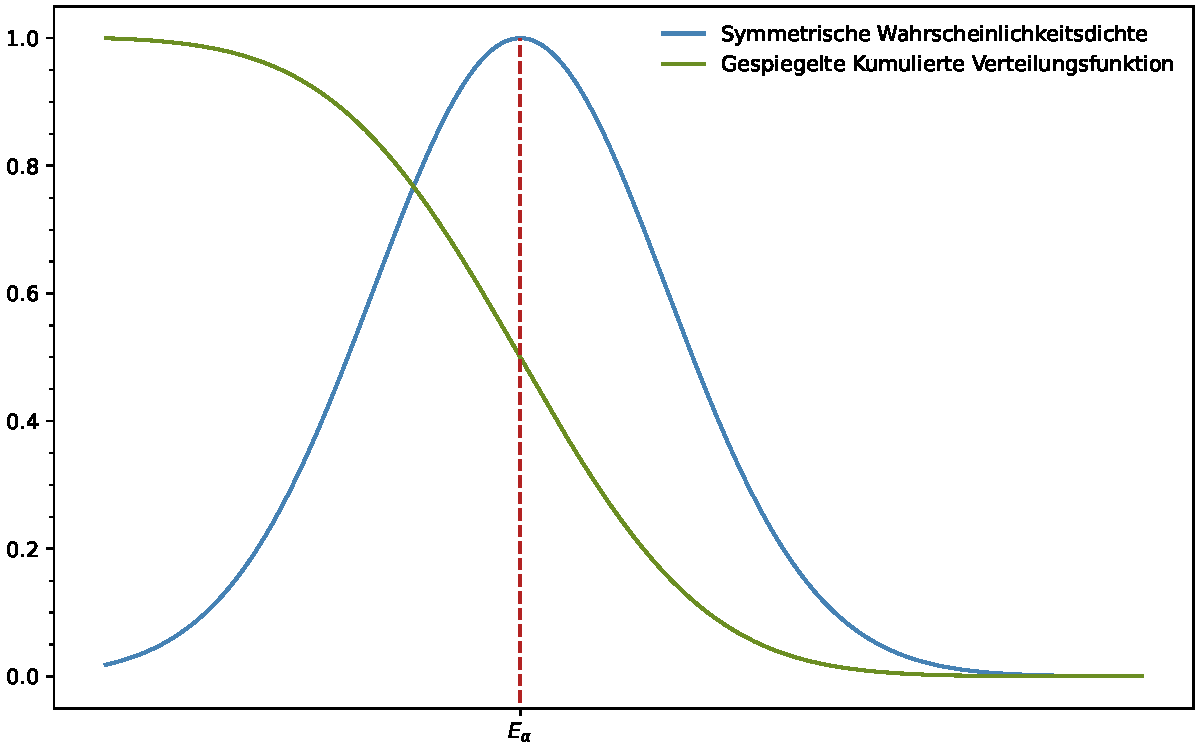
\includegraphics[width=1\textwidth]{content/messung/EnergiePuls.pdf}
    \caption{Druckabhängigkeit der Energie der $\alpha$-Strahlung.}
    \label{fig:EnergiePuls}
\end{figure}

In Formeln niedergeschrieben, bedeutet das 
\begin{align*}
U &= a \cdot p + b & p &= \frac{U - b}{a} & \Delta E = E_\alpha \, \frac{\Delta p}{p_\alpha}
\end{align*}
Aus den Messdaten folgen 
\begin{align*}
U_{\alpha} &= 6.05\, \text{V}\\
p_{\alpha} &= (165\pm 5)\, \text{mbar}\\
\Delta p &= (66\pm 6)\ \text{mbar}\\
E_{\alpha} &= 5.5\, \text{MeV}\\
\Delta E &= (2.2\pm 0.2)\, \text{MeV}\\
\end{align*}

Wird dies in die Bethe-Bloch-Gleichung \ref{eqn:Bethe} eingesetzt und nach $\Delta x$ umgestellt, folgt
$$d = \Delta x_\alpha = \Delta E_\alpha \frac{4\pi m_e v_\alpha^2 \varepsilon_0^2}{e^4 N z^2 Z \ln (2m_e v_\alpha^2 / I)}
= \Delta E_\alpha \frac{8\pi m_e E_\alpha \varepsilon_0^2}{m_\alpha e^4 N z^2 Z \ln (4m_e E_\alpha / m_\alpha I)} = (5.1\pm 0.4) \, \unit{\micro \meter}
\; .$$